\chapter{实验与评估}
\label{ch5}
之前的章节中,我们描述了联邦学习的本地自适应差分隐私和安全混洗模型的设计和实现过程。在本节的内容中,我们选取了一些基准的数据集在该验证框架上进行实验评估。本章的实验主要针对联邦深度学习系统训练样本的攻击模型,保护联邦学习系统中参与者的共享梯度信息,避免梯度参数泄露隐私和恶意服务器获取客户端的信息,进而保护参与者本地训练样本。在实验室环境下,通过多 GPU 虚拟化设置模拟分布式联邦学习系统,并且将差分隐私保护方案和混洗器配置在模拟分布式联邦学习系统中,同时在系统中设置攻击模型,评估满足隐私保护算法的系统学习准确率和隐私保护预算。 
\section{基准数据集介绍}
我们选用以下三个数据集评估了我们的联邦学习隐私保护框架:
\begin{enumerate}
	\item [(1)] 手写体数字识别数据集(MNIST)\upcite{ref46}是用于分类任务的经典数据集,来源于美国国家标准与技术研究所。总共包含了70000个尺寸为28 x 28像素的手写数字图像,每个像素点用灰度值表示,灰度值范围为0到255,图像包含十个类别。
	\item [(2)] FASHION-MNIST 数据集包含了 70000 个不同商品的正面灰度图像,与 MNIST 数据集一样,每个图像的尺寸为28x28像素,灰度值范围同样为0到255。所有的图像分为10种类别,如:T恤,牛仔裤,裙子等。虽然数据集格式与 MNIST 相同,但由于图像内容的差别,使得有些模型或者算法在MNIST和FASHION-MNIST的表现会有很大不同。
	\item [(3)] CIFAR-10数据集包含了10类(飞机、汽车、鸟类、蛙类、卡车、船、马、猫、鹿、狗)32x32的彩色图片,一共有60000张,每一类包含6000张图片。该数据集按照5:1的比例划分成了5个训练的batch和1个测试的batch。

\end{enumerate}

\section{实验环境与配置}
本文中的所有的实验是在 Windows 10 系统下,使用 CPU Inter(R) Core i3-7100 @ 3.90GHz,GPU的型号是 NVIDIA GeForce GTX1050,内存8GB。在实验中使用了Facebook公司的Pythorch框架对神经网络模型进行编写,相比于TensorFlow,PyTorch 网络定义方便,更有利于研究小规模项目快速做出原型。其对于并行化数据的支持更有利于分布式联邦系统的实验等)。在对样本数据预处理的部分,我们使用了Pandas,Numpy 等第三方库。

\section{实验设计}
\subsection{联邦学习模型}
实验设置了30 名联邦学习的参与者,论文研究在分布式联邦系统中添加噪声达到差分隐私并使得整体模型的精度维持较优。首先考虑了如何设置超参数可以更好的让全局模型能够得到更好的训练。
分布式联邦学习梯度选择的准则是选择差值变化最大的, 调整梯度上传阈值, 将上传比例 $\theta_{u}$ 设置为 $0.1$, 将从参数服务器下载的全局参数的比例 $\theta_{d}$ 设置为 1。

接下来,在联邦系统中实施本文所提出隐私保护方案。实验设置每个参与者在训练分布式联邦系统时每次迭代的总隐私预算为 $\epsilon$, 将隐私预算分成 $c$ 个部分, 其中 $c$ 是选择每次迭代满足神经网络前向传播算法的梯度总数, 即 $c=\theta_{u}|\Delta w|$ 。我们使用拉普拉斯机制根据分配的隐私预算在选择梯度过程中添加噪声。添加的噪声取决于隐私预算所有参数的灵敏度 $\Delta f$,不同的参数可能导致函数的灵敏度不同。 

在分布式联邦学习模型中,实验评估了不同$\frac{\theta_{u}}{\theta_{c}}$ 值的情况下($\theta_{u}$为选择梯度阈值的参数), 使用论文方案满足差分隐私的分布式联邦系统能达到的全局模型准确率, 并且将添加隐私保护后的系统精度与未添加隐私保护的模型精度相比较。

\subsection{神经网络模型}
Shokri\upcite{ref51}等人在论文中公开了他们的源代码,实现了一个完整的分布式联邦学习系统。我们将攻击模型部署在该联邦系统中,并且使用其中的卷积神经网络(CNN)架构,如图\ref{fig:卷积神经网络结构图}。在CNN架构中,网络的前端是卷积层和池化层,后端则是使用反向传播算法的全连接层。前端的网络结构是在一个nn. SpatialConvolution 卷积层连接激活函数 TanH,后面再接一个 nn.SpatialMaxPooling 最大池化层。之后再连接卷积层、TanH 激活函数和池化层单元。后端的网络架构则是 nn.Linear 线性层加上 TanH 激活函数和分类输出层。CNN 网络结构中的参数个数计算如下:
$$
32×5×5 + 32 + 64×32×5×5 + 64 + 200×256 + 200 + 10×200 + 10 = 105506
$$

\begin{figure}[!hbt]
\centering
  	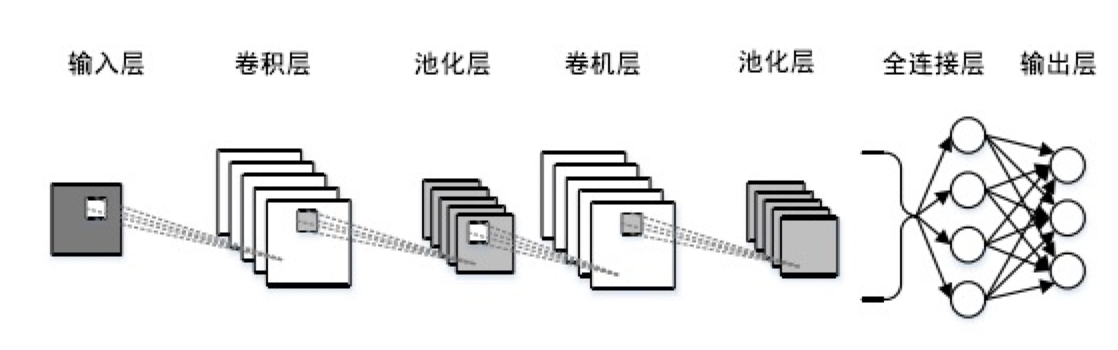
\includegraphics[scale=0.6]{fig2/C5/CNN结构}%联邦学习的系统架构
	\caption{卷积神经网络结构图}
  	\label{fig:卷积神经网络结构图} 
\end{figure}

CNN 网络中的损失函数为 nn.CrossEntropyLoss。该函数是nn.NLLLoss 和\\nn.LogSoftmax 的结合,激活函数使用 Softmax 函数,损失函数使用交叉熵损失函数评估模型的损失,也更便于计算反向传播算法。在选择梯度上传的全连接层与传输协议中, 部分超参数选择如下: 选择参数比例 $\theta_{u}=0.01$, 全局参数 $\theta_{d}$ 下载比例为 1 。为了展现学习模型的随机性, 将学习率设置为 $\alpha=1 \times 10^{-2}$, 学习速率衰减值为 $1 \times 10^{-7}$ 。参与者迭代过程使用CNN训练本地数据集,攻击者使用基于 CNN 网络的 DCGAN算法与成员推理攻击的白盒算法。实验在这样的参数设置下搭建一个包含 29 个正常参与者和 1 个攻击者的 分布式联邦学习系统, 30 个参与者(包含攻击者)都与中央参数服务器进行连接。

实验中使用60000 条数据作为训练数据集,每一个客户端拥有 10 个样本的数据,剩下的样本则作为测试数据集,每种情况分别重复做 5 次并取平均值。实验通信迭代次数为T = 200,步长 α = 1e − 4 ,衰减系数 γ = 0.99。

\section{自适应扰动方案的实验评估}
针对第三章提出的自适应扰动框架,我们从模型预测的准确率和隐私预算参数$\epsilon$两个角度评估该方案,隐私预算参数越小,意味着隐私保护的力度越大;模型的准确率越高意味着模型的可用性越高。我们分别使用梯度固定加躁方法和梯度自适应加躁方法进行实验,实验结果如下。

(1)使用梯度固定加噪方法:在公共数据集上进行训练,每轮迭代过程中,在训练批次大小L=600个样本中添加噪声,因此采样率为为$\mathrm{q}=\frac{L}{N}=\frac{600}{60000}=0.01$。在采集的训练样本中添加的噪声量为σ = 5,隐私参数为$\delta=10^{-5}$,固定的梯度裁剪阈值为0.001。如图\ref{fig:梯度固定加噪方法下模型准确率随隐私预算变化情况}所示,隐私预算参数ε为研究变量。隐私预算代表着隐私保护强度,两者呈负相关的关系。隐私预算越大意味着添加的噪声量越小,隐私保护的强度越低,模型的精度越高,符合上文的理论分析。当隐私预算$\frac{\epsilon}{c}$≥ 5后,隐私预算参数对于模型准确率影响趋于平稳,综合来看,当$c$≥ 7后,部署了差分隐私机制的模型准确率能达到90$\%$左右,与原始不加噪声的模型相比,准确率下降了7$\%$。
\begin{figure}[!hbt]
\centering
  	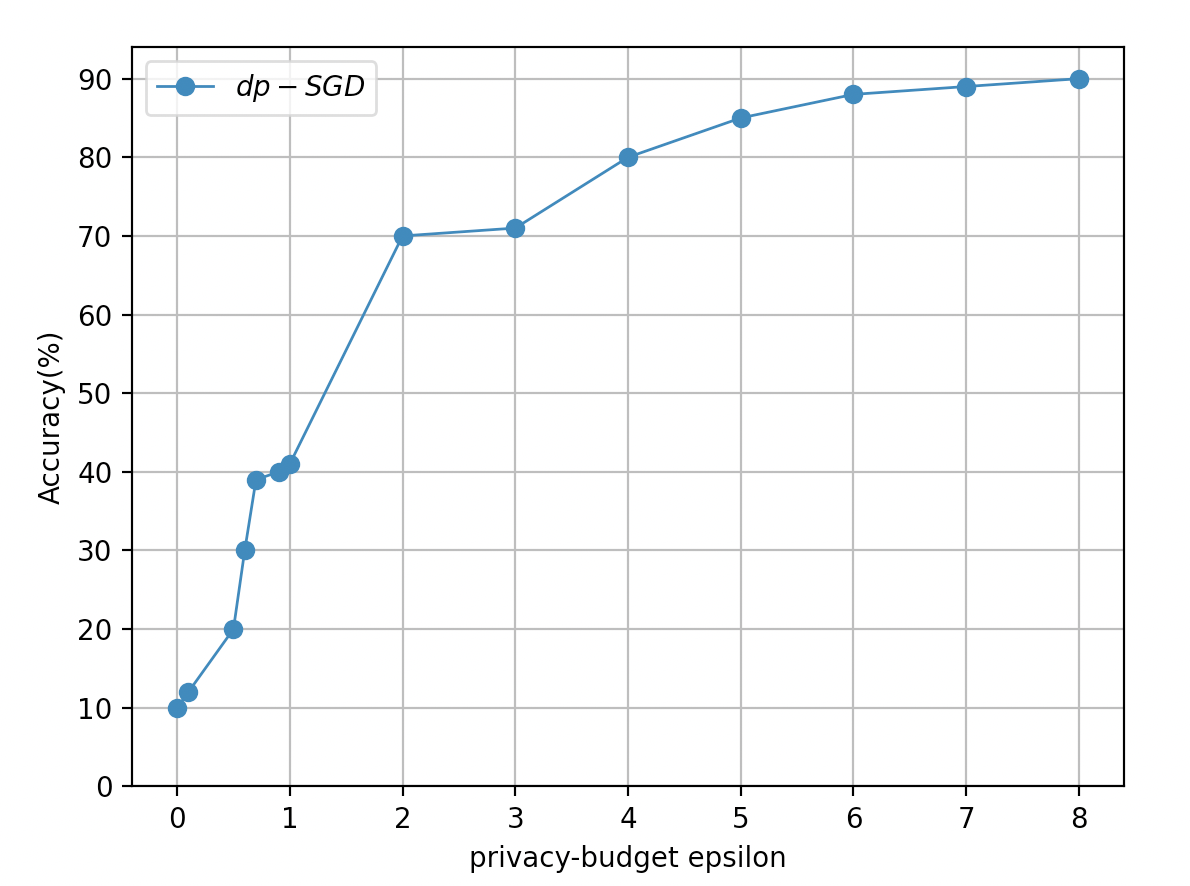
\includegraphics[scale=0.4]{fig2/C5/梯度固定}%联邦学习的系统架构
	\caption{梯度固定加噪方法下模型准确率随隐私预算变化情况}
  	\label{fig:梯度固定加噪方法下模型准确率随隐私预算变化情况} 
\end{figure}

(2)使用梯度自适应扰动方法:之后我们比较了在不同隐私预算下的自适应干扰模型的准确性,隐私预算分别为($\epsilon$1 = 0.1, $\epsilon$2 = 0.5, $\epsilon$3 = 2.0, $\epsilon$4 = 8.0)。
隐私预算$\epsilon$越小,噪音就越大。我们还为每个隐私预算选择三种不同的超参数设置(a): f = 0.15, p = 0.85, (b): f = 0.10, p = 0.90 (c): f = 0.05, p = 0.95。在实验中,隐私预算ε的值是εc、εl和εc的总和。我们将隐私预算的计算分为以下三个步骤:对于贡献的计算、线性转换中的计算和
损失函数的计算,即:$\epsilon_{c}=\epsilon_{l}=\epsilon_{f}=\frac{\epsilon}{3}$。

正如图\ref{fig:不同隐私预算的自适应干扰机制在MINIST数据集上的准确率}所示,随着隐私预算ε的增加,我们系统的准确性保持稳定的增长趋势。随着调整因子范围的不断缩小,自适应干扰模型的准确率逐渐降低,但仍保持较高的水平。例如,当隐私预算ε设置为8.0时,在f=0.15和p=0.85的设置下,自适应差分隐私联邦学习模型的准确率高达97.34$\%$,而在f=0.10和p=0.90的设置下,准确率为96.57$\%$,以及在f=0.05和p=0.95的设置下,准确率为96.25$\%$。

\begin{figure}[!hbt]
\centering
  	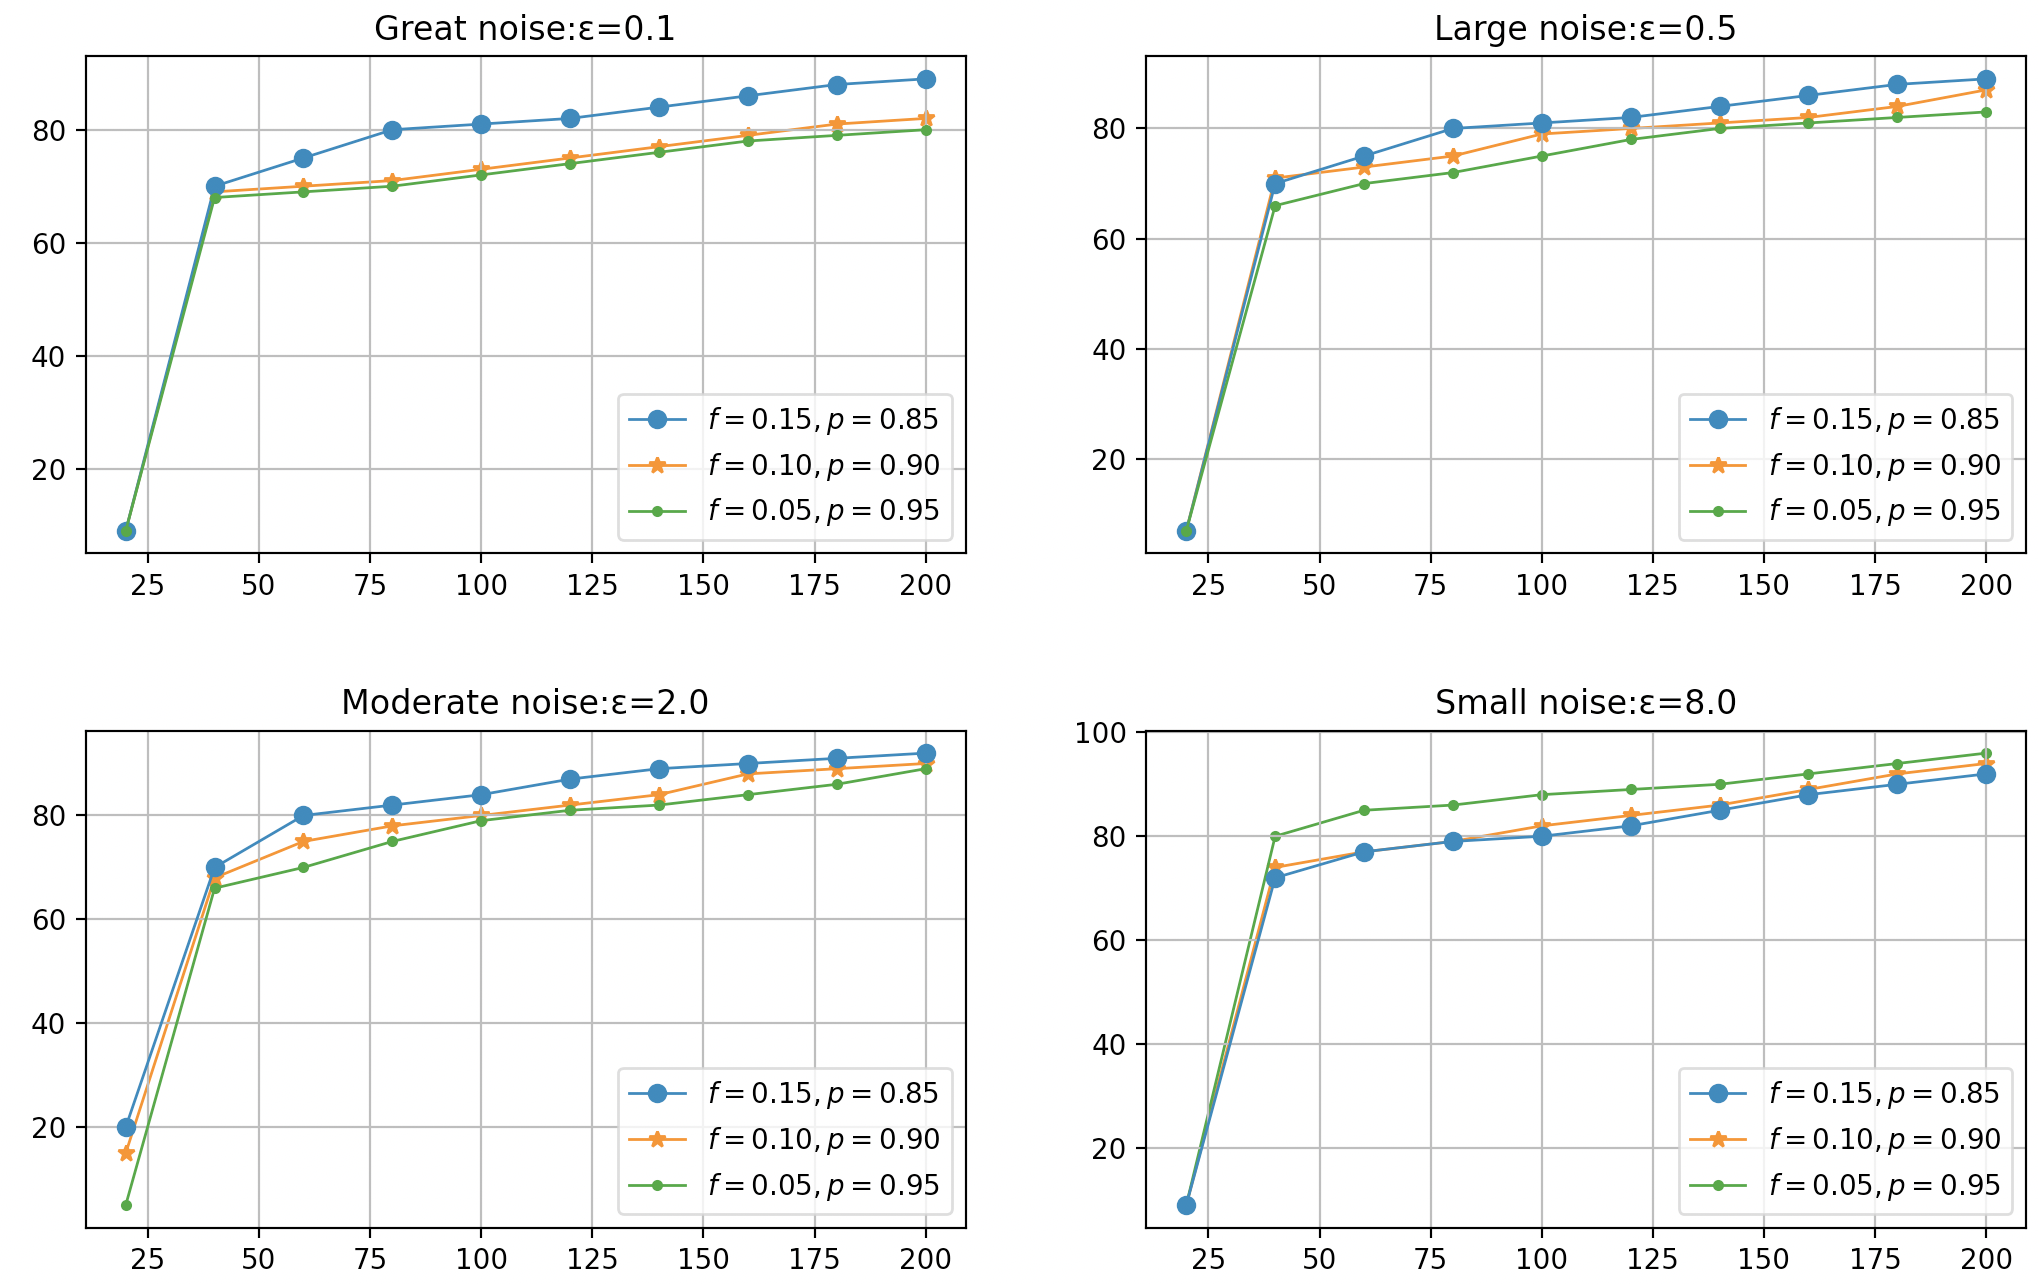
\includegraphics[scale=0.4]{fig2/C5/自适应干扰实验}%联邦学习的系统架构
	\caption{不同隐私预算的自适应干扰机制在MINIST数据集上的准确率}
  	\label{fig:不同隐私预算的自适应干扰机制在MINIST数据集上的准确率} 
\end{figure}

综上,自适应隐私预算分配可以根据模型训练的收敛规律,合理地分配隐私参数,从而提高模型表现,但隐私预算参数需要小心选取,过大的隐私预算参数会导致训练的初始阶段噪声太大,从而影响模型的可用性。

我们还与近年来使用差分隐私机制保护深度学习模型隐私的工作(DLPP和DP-SGD)进行了比较。从图\ref{fig:DP-SGD、DLPP、ACDP-SGD在模型准确率和隐私预算上的对比}不难发现我们的方案(ACDP-SGD)即使在强隐私预算下(ε=0.1)也表现良好。当调整因素设置为f = 0.15和p = 0.85时,模型的准确率在200个通信回合后还能达到88.46$\%$。此外,调整因素为f=0.05和p=0.95,自适应干扰模型的准确率为86.79$\%$。然而,在相同的隐私预算下,差分隐私随机梯度下降算法(DP-SGD)\upcite{ref45}的准确性仅达到79.63$\%$,本地差分隐私DLPP模型的准确性低于65.00$\%$。

\begin{figure}[!hbt]
\centering
  	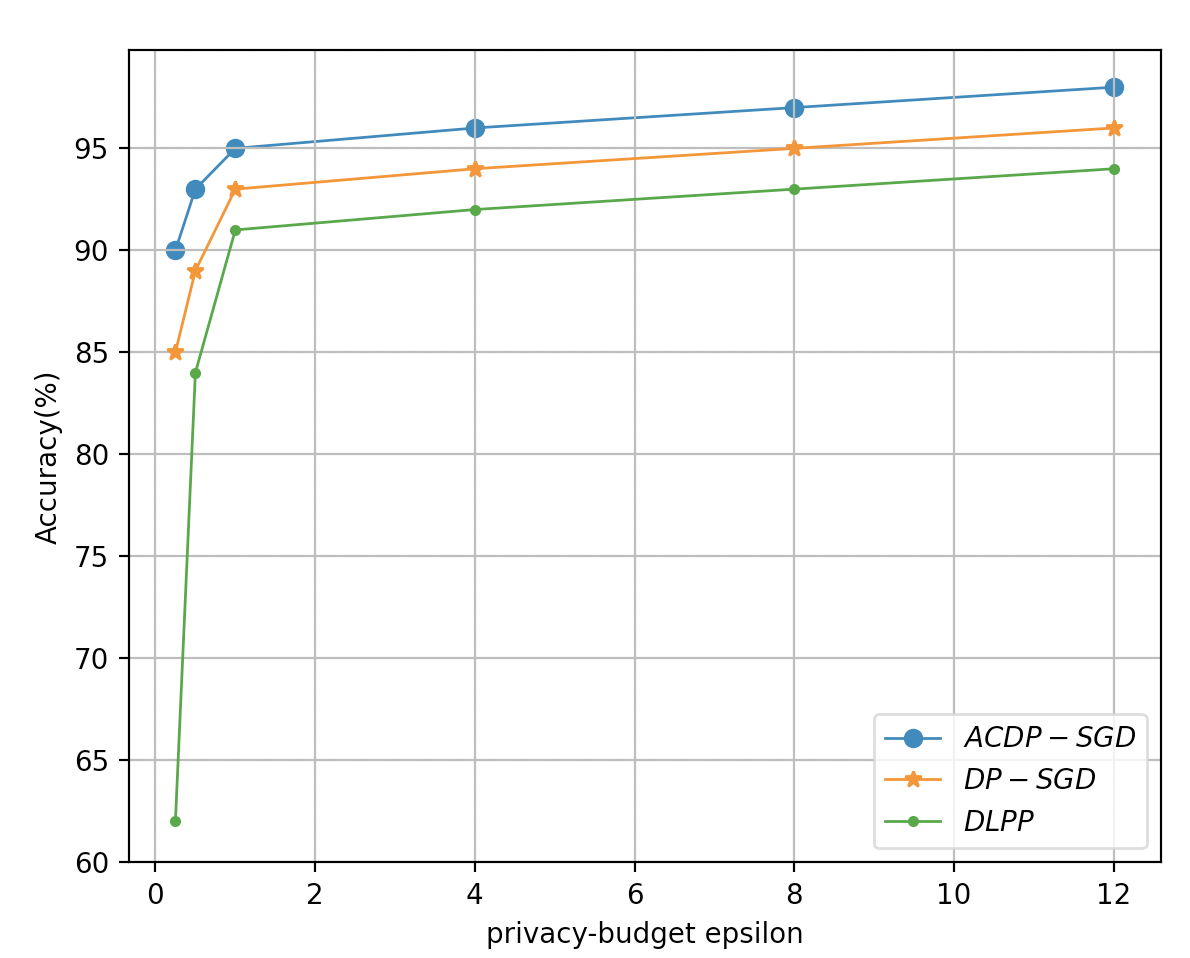
\includegraphics[scale=0.4]{fig2/C5/自适应干扰实验对比}%联邦学习的系统架构
	\caption{DP-SGD、DLPP、ACDP-SGD在模型准确率和隐私预算上的对比}
  	\label{fig:DP-SGD、DLPP、ACDP-SGD在模型准确率和隐私预算上的对比} 
\end{figure}


\section{安全混洗算法的实验评估}
我们在MNIST、FMNIST和CIFAR上评估所提出的安全聚合框架。首先评估参数:客户端数量$n$对于隐私预算和模型预测准确率的影响。如图\ref{fig:安全混洗模型中参与混洗的本地客户端数量对联合模型精度的影响}所示,通过客户端采样机制和梯度的拆分混洗算法,我们的安全混洗模型(下文简称SA-FL)能够以较低的隐私成本实现较高的准确性。在训练中增加客户数量n的同时,SA-FL能达到的模型精度与不添加噪声的联邦学习几乎接近。与MNIST(n=100,ε=1)、FMNIST(n=200,ε=5)相比,CIFAR-10(n=500,ε=10)需要更多的客户端,这表明对于一个具有较大神经网络模型的更复杂的任务,当在更多的本地数据和更多的客户端上添加扰动之后,需要更多的通信回合才能使联合模型达到更高的精度。

\begin{figure}[!hbt]
\centering
  	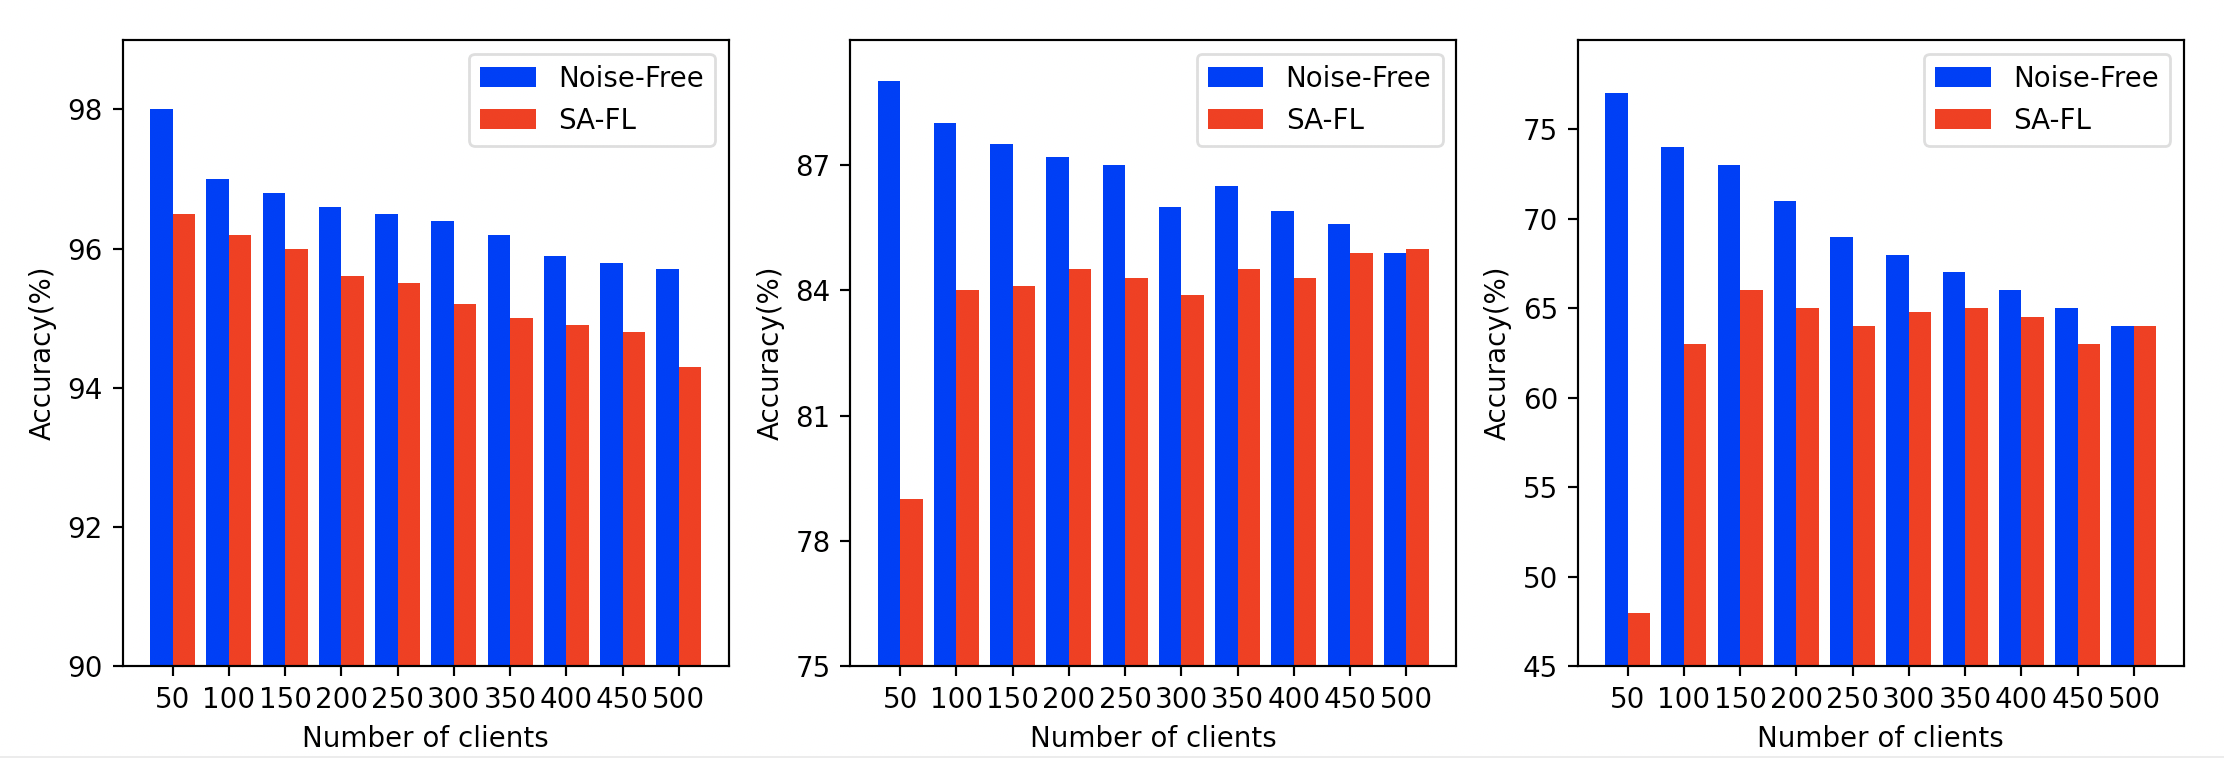
\includegraphics[scale=0.37]{fig2/C5/SA-FL}%联邦学习的系统架构
	\caption{安全混洗模型中参与混洗的本地客户端数量对联合模型精度的影响}
  	\label{fig:安全混洗模型中参与混洗的本地客户端数量对联合模型精度的影响} 
\end{figure}

接着,我们分别在MNIST, FMNIST和CIFAR-10数据集上评估了客户端采样比$f_{r}$和通信回合$m$对于模型训练准确率的影响。由图\ref{fig:安全混洗模型中通信轮数和客户端采样比对联合模型精度的影响}可以发现,当$f_{r}$太小的时候,并不影响在MNIST上的表现,但对FASHION-MNIST和CIFAR-10的表现影响很大。当$f_{r}$接近1时,安全聚合框架可以在MNIST、FASHION-MNIST和CIFAR-10上达到与不添加噪声的联邦学习模型几乎相近的性能。另一个重要的参数是中央参数聚合器和本地客户端之间的通信轮次$m$。不难看出,随着通信次数的增加,我们可以通过所提出的模型在所有数据集上训练出更好的模型。然而,由于数据和任务的复杂性,CIFAR-10需要更多的通信回合以获得更好的模型。

\begin{figure}[!hbt]
\centering
  	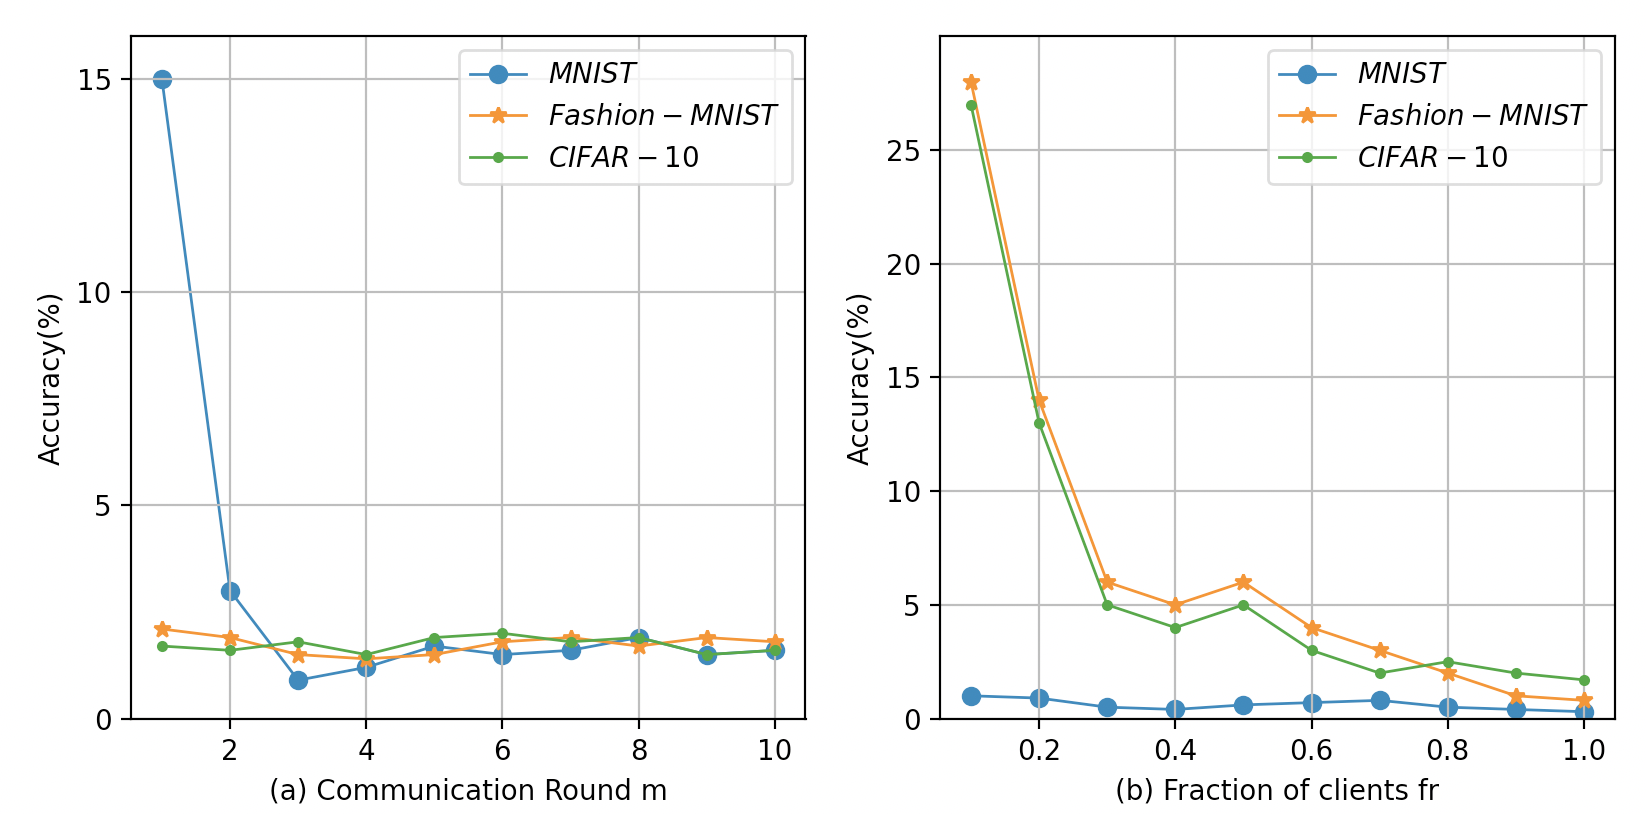
\includegraphics[scale=0.4]{fig2/C5/SA-FL2}%联邦学习的系统架构
	\caption{安全混洗模型中通信轮数和客户端采样比对联合模型精度的影响}
  	\label{fig:安全混洗模型中通信轮数和客户端采样比对联合模型精度的影响} 
\end{figure}

最后,我们统一比较应用了自适应差分隐私算法和安全混洗器的联邦学习模型与其他联邦学习隐私保护模型,在相同隐私预算参数下训练模型能达到的精度。如图\ref{自适应差分混洗模型和其他联邦学习隐私保护模型的比较}(a-c)中,SA-FL在ε=4和n=100的情况下可以达到96.24$\%$的准确率,在ε=4,n=200的情况下可以达到86.26$\%$的准确率,在ε=10,n=500的情况下,在MNIST,FMNIST和CIFAR-10上可以达到61.4$\%$的准确率。我们的结果与之前的其他工作相比非常有竞争力。Geyer等人\upcite{ref53}首次将差分隐私应用于联邦学习,虽然他们只使用了100个客户端,但在MNIST上,他们只能在(ε,m)=(8,11),(8,54)和(8,412)的情况下达到78$\%$,92$\%$和96$\%$的准确率,其中(ε,m)代表隐私预算和通信回合。Bhowmick等人\upcite{ref54}首次在联合学习中利用本地差分隐私。由于其机制的高变异性,它需要超过200轮的通信回合和更高的隐私预算才能使模型收敛。最近,Truex等人\upcite{ref55}将压缩后的局部差分隐私(α-CLDP)应用到联邦学习中,在FMNIST数据集上获得了86.93$\%$的准确性。然而,α-CLDP需要相对较大的隐私预算ε = α-2c-10ρ(例如,α = 1,c = 1,ρ = 10)来实现模型的收敛,这导致了方案的隐私保证程度太低。与以往的工作相比,我们的方案大大减少了客户端和中央服务器之间需要的通信回合(例如,MNIST为10,FMNIST和CIFAR-10为15就能达到全局模型收敛),这使得整个解决方案在实际场景中更加实用。总的来说,SA-FL在隐私成本、模型精度和通信成本方面都比之前的作品取得了更好的表现。

\begin{figure}[!hbt]
\centering
  	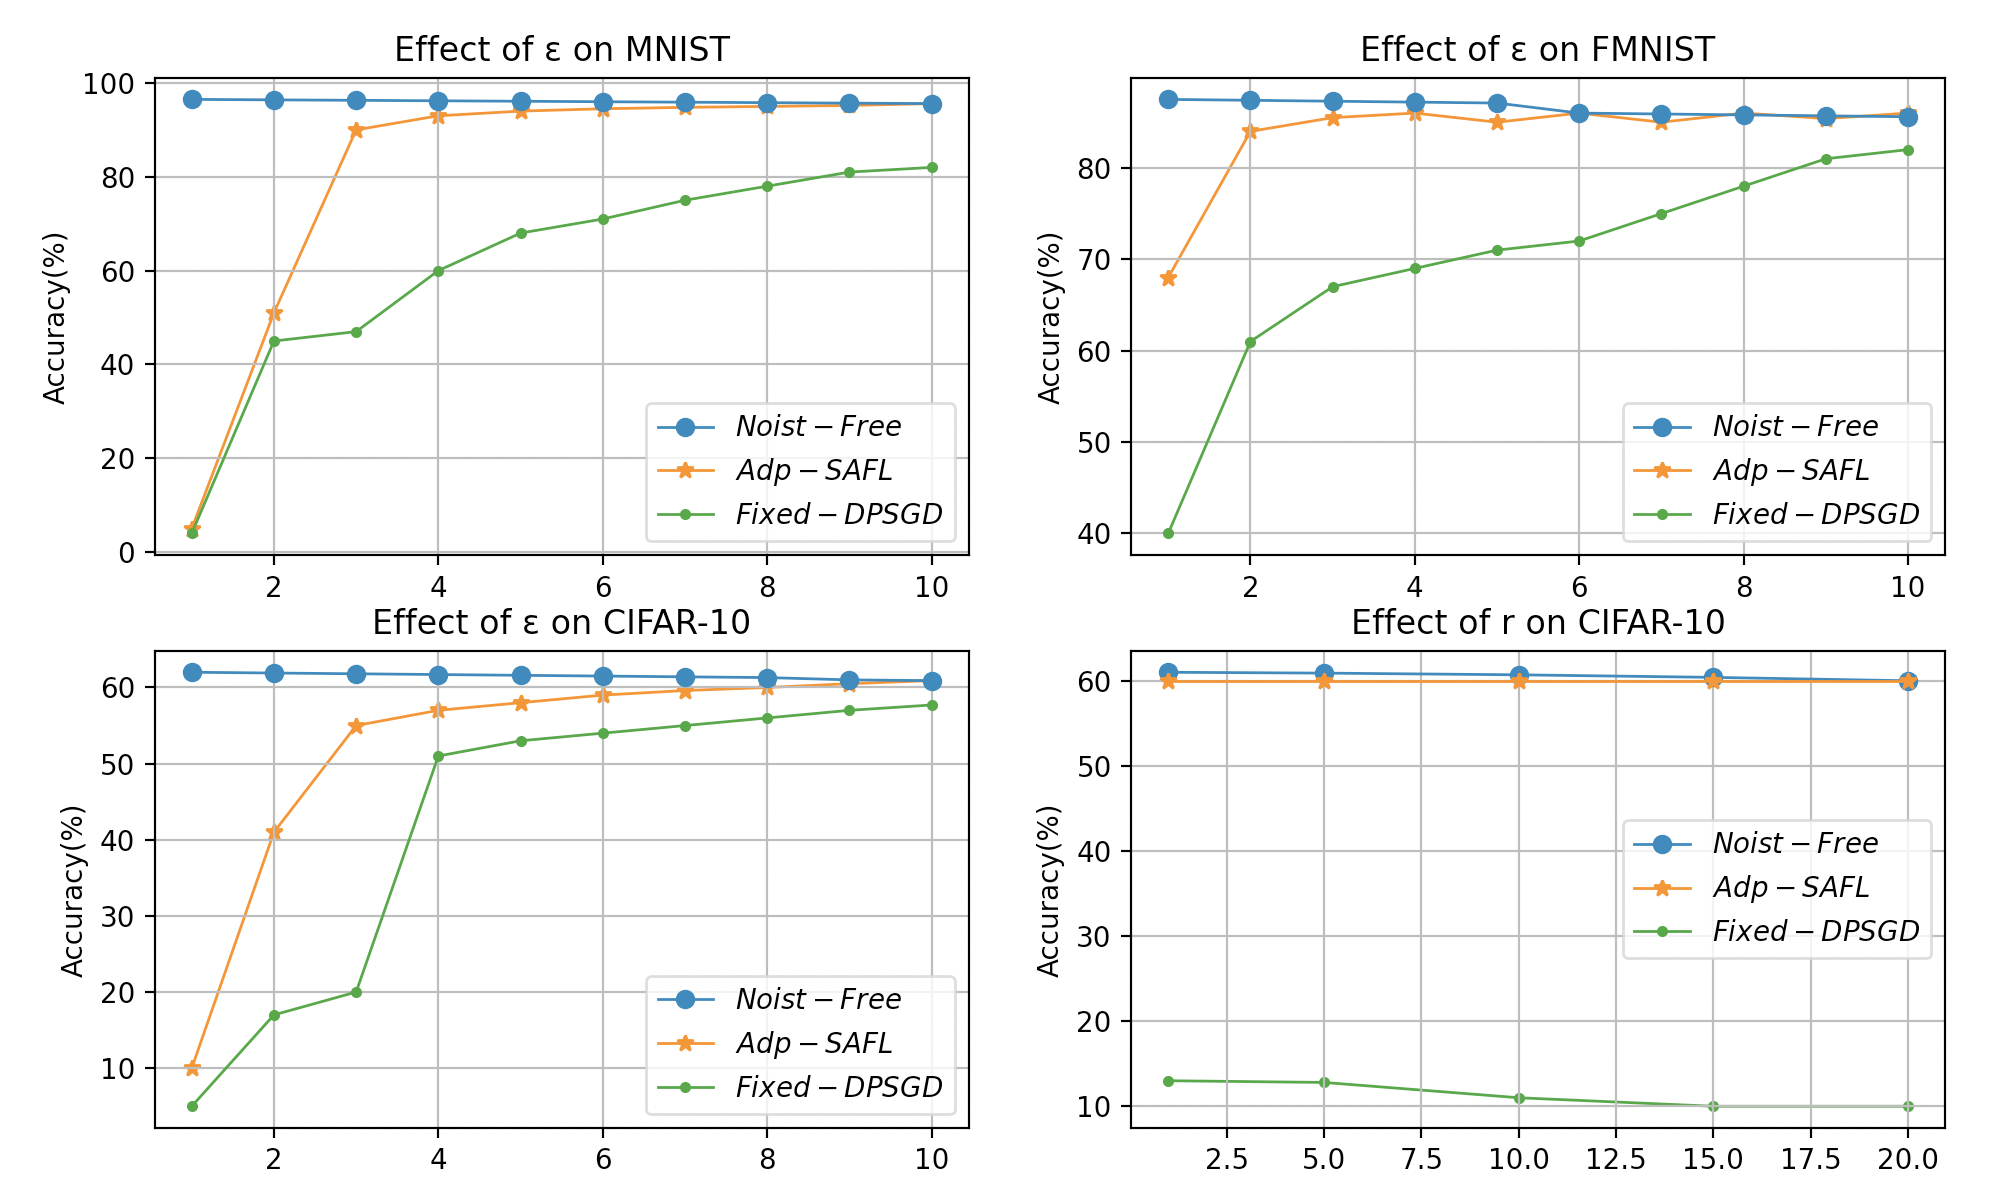
\includegraphics[scale=0.4]{fig2/C5/SA-FL对比实验}%联邦学习的系统架构
	\caption{自适应差分混洗模型和其他联邦学习隐私保护模型的比较}
  	\label{自适应差分混洗模型和其他联邦学习隐私保护模型的比较} 
\end{figure}

\section{结果分析}
为了验证自适应扰动算法在隐私保护的同时,也能使模型训练的精度维持在较优的水平,我们进行了对比实验,使用自适应扰动算法和使用固定加躁方法在不同的隐私参数$\epsilon$下进行对比实验。由本章第三节对于自适应差分隐私方案的实验评估,我们可以看到自适应
扰动算法基本上占有绝对的优势,尤其是损失函数值,在隐私参数$\epsilon$=0.1时,我们的方法不到1,而传统的平均算法却在100左右。这么大的差距的原因在于,自适应扰动算法的权重分配使得参数聚合时个体信噪比不变,但整体的聚合结果的信噪比却提高了很多,因此当隐私参数$\epsilon$很小,即噪声量很大的时候,表现越好。而当$\epsilon$越大时,注入的噪声也就越小,自适应加躁方法的效果就没有噪声大的时候明显。

联邦学习系统的额外开销主要来自服务器端的预训练过程,以及用户端在开始训练前对权重贡献率的计算和梯度的扰动。我们使用20个通信回合来训练中央服务器的初始化模型,这平均需要68.22秒。在本地模型的训练开始之前,用户需要使用前向传播算法计算权重。这个过程只需要训练神经网络前向传播算法,而不需要训练反向传播来计算损失函数,进行梯度下降,其平均耗时为4.35毫秒。
为了减轻隐私威胁,我们提出的解决方案是向权重、线性变换函数中的原始数据和损失函数的系数注入拉普拉斯噪声。向权重注入噪声的步骤可以与计算权重的贡献率同步进行,这需要额外的2.67毫秒时间。向线性变换中的原始数据和损失函数的系数注入自适应噪声的操作可以在训练前完成。因此,在模型效率方面的提升是非常突出的。

从隐私成本和模型精度的总体上看,混洗差分隐私方法在各统计问题的结果可用性上都有着相比本地化差分隐私方法明显更优的结果。但从通信代价和计算代价的角度分析,安全混洗算法中混洗器的引入,使得用户数据与用户所使用的编码器之间的关联性消失,使得中央服务器的计算代价增大。如何兼顾数据的隐私性、可用性、算法的计算代价和通信代价是后续基于SA-FL框架构建隐私保护方法需加以研究的部分。

在本节中,我们根据图像基准数据集MNIST、Fashion-MNIST(FMNIST)来研究不同权重的效果,然后根据CIFAR-10来验证性能的提升。对于MNIST和FMNIST,我们实现了一个两层的CNN进行图像分类。然而,对于CIFAR-10,Pytorch库的默认网络在没有数据扰动的情况下只能达到\%左右的准确率,因此我们重新设计了一个小型的VGG网络来完成这个任务。训练数据和测试数据直接输入每个客户端的网络,对于每个客户端,训练数据的大小是训练样本的总数除以客户端的数量。在这种情况下,客户数量越多,说明每个客户的训练数据规模越小。对于每个权重,我们把它们夹在一个固定的范围内。在这项工作中,我们为MNIST和FMNIST分别默认设置(c,r)=(0,0.075)和(0,0.015)。然而,对于CIFAR-10,由于模型的复杂性,我们没有使用固定的范围,而是通过每层的权重范围自适应地设置c和r。对于MNIST/FMNIST,学习率γ被设定为0.03,对于CIFAR-10,学习率γ被设定为0.015。考虑到扰动过程中的随机性,我们独立地运行了十次测试实验以获得一个平均值。为了评估不同学习方法的性能,我们使用了不同的指标,包括效用的准确性、隐私成本的ε和通信成本的m,即通信轮数。任何具有高精确度、小的ε和小的通信回合的方法都表明是一个好的和实用的解决方案。所提出的模型是用Pytorch实现的,所有的实验都是在本地服务器上用单个GPU NVIDIA Tesla V100完成的。对MNIST和FMNIST的实验在10个CR的情况下可以在一小时内完成,而对CIFAR-10的实验在15个CR的情况下需要2个小时左右。

我们设计了实验来评估所提出的混洗器的性能,在实验中,我们衡量了
\begin{enumerate}
\item [(1)] 所提出的协议的准确性,即它们比现有的洗牌协议提高了多少准确性;
\item [(2)] 所提出的协议的通信开销,即每个用户需要发送多少信息;以及它们与现有的洗牌协议相比如何
\item [(3)] 关键参数如何影响提议的协议的准确性,即本地用户数n和通信回合cr;为了实现这些目标,我们在合成和真实世界的数据集上进行了实验。合成数据集允许我们调整数据集的关键参数,以观察其对协议效用的影响。而真实世界的数据集将显示所提出的协议在一个更实际的环境中的效用。
\end{enumerate}


\section{本章小结}
在本章中,我们选取了三个基准数据集对本文提出的自适应本地差分隐私和安全混洗框架进行了一系列的实验来测试其可行性,并且在联邦学习系统上也进行实验和研究。实验结果表明,我们的自适应本地差分隐私方案可以有效降低隐私预算,并且维持模型精度。安全混洗框架能通过客户端采样算法和梯度的拆分混洗算法,降低隐私保护预算,提高数据的可用性。

